\documentclass[12pt,twoside]{article}
\usepackage{graphicx}
\usepackage{jmlda}
%\NOREVIEWERNOTES
\title
    [Задача поиска символов в текстах] % Краткое название; не нужно, если полное название влезает в~колонтитул
    {Задача поиска символов в текстах}
\author
    [Северилов~П.\,А.] % список авторов для колонтитула; не нужен, если основной список влезает в колонтитул
    {Северилов~П.\,А., Лемтюжникова~Д.\,В., Апишев~М.\,А.} % основной список авторов, выводимый в оглавление
    [Северилов~П.\,А.$^1$, Лемтюжникова~Д.\,В.$^1$, Апишев~М.\,А.$^2$] % список авторов, выводимый в заголовок; не нужен, если он не отличается от основного
\thanks
    {
    	%Работа выполнена при финансовой поддержке РФФИ, проект \No\,00-00-00000. Научный руководитель:  
   Задачу поставил:  Лемтюжникова~Д.\,В., 
    Консультант: Апишев~М.\,А.}
\email
    {severilov.pa@phystech.edu, daratigra@icloud.com, great-mel@yandex.ru}
\organization
    {$^1$Московский физико-технический институт (МФТИ); 
    	
	 $^2$Московский государственный университет имени М.В.Ломоносова (МГУ им. М.В.Ломоносова)}
\abstract
    {В работе рассматривается задача поиска символов в тексте. Определение в тексте средств выразительности  таких, как метафоры, аллегории и пр. у экспертов происходит в ручном режиме, и процесс никак не автоматизирован. В простейшем случае эта задача сводится к проблеме Sequence Labeling на размеченной выборке. Сравниваются работы современных алгоритмов решения Sequence Labeling и определяется применимость данных методов к задаче. %Также предложена метрика качества классификатора для определения символ/не символ.

\bigskip
\textbf{Ключевые слова}: \emph {распознавание символов, LSTM нейронные сети, sequence labeling, cкрытые марковские модели}.}
\titleEng
    {JMLDA paper example: file jmlda-example.tex}
\authorEng
    {Author~F.\,S.$^1$, CoAuthor~F.\,S.$^2$, Name~F.\,S.$^2$}
\organizationEng
    {$^1$Organization; $^2$Organization}
\abstractEng
    {This document is an example of paper prepared with \LaTeXe\
    typesetting system and style file \texttt{jmlda.sty}.

    \bigskip
    \textbf{Keywords}: \emph{keyword, keyword, more keywords}.}
\begin{document}
\maketitle
%\linenumbers
\section{Введение}
Современные модели для обработки текстов не справляются с главной особенностью языка — неоднозначностью смысла высказывания. Текст воспринимается ими буквально, и различные средства художественной выразительности, в частности, символы, метафоры, аллегории и др. не интерпретируются очевидным образом. Так, например, выражение «золотые руки» вероятнее всего будет понято моделью, как «руки из золота» вместо верного «умения очень хорошо делать что-либо». Автоматизация поиска выражений с неоднозначным смыслом продвинет механизм обработки текстов на другой уровень абстракции.

Задача поиска символов в тексте может быть сведена к sequence labeling -- более общей задаче, широко распространенной в NLP. Как правило, рассматриваются три конкретных типа sequence labeling: тегирование частей речи (part-of-speech tagging), распознавание именованных сущностей (named entity recognition) и синтаксический анализ (shallow parsing). Данные методы могут быть применены к текущей задаче.

Традиционно задачи sequence labeling решаются с использованием линейных статистических моделей, например: скрытые марковские модели (HMM), марковские случайные поля (CRFs). Реализация решений происходит с помощью различных архитектур нейронных сетей. В данной статье сравниваются результаты работ нескольких state-of-the-art архитектур для sequence labeling применительно к задаче поиска символов. 

Архитектуры таких нейронных сетей главным образом базируются на рекуррентных сетях, а именно Bidirectional LSTM с использованием CRF. Рассматривается три подхода. Первый -- это классическая реализация BiLSTM. Затем предложена следующая модификация: на вход сети будут подаваться не векторные представления слов в целом, а каждый символ по отдельности. И третий подход -- основан на предыдущей модели, но с интеграцией механизма внимания (attention) в архитектуру. %(Transformer).

Чтобы определить скрытый смысл высказывания, для начала необходимо ответить на вопрос, есть ли он вообще в нём. Поэтому решается задача классификации символ/не символ. Тестирование проводится на тексте романа М. А. Булгакова "Мастер и Маргарита" и стихотворных текстах поэтов серебряного века. Основная сложность заключается в получении достаточного объёма обучающих данных, то есть требуется по имеющейся небольшой экспертной разметке получить выборку большего размера. Наличие разметки позволит провести эксперименты с подбором оптимальной модели и в целом определить применимость данных методов для решения задачи поиска символов.
%\cite{author09anyscience,myHandbook,author09first-word-of-the-title,voron06latex,author-and-co2007,Lvovsky03}.

\section{Постановка задачи}
Рассматривается два подхода к задаче: с точки зрения классификации и с точки зрения sequence labeling.

\begin{enumerate}
	\item \textbf{Sequence labeling}: Дано предложение \textbf{X}, разделенное на части (слова): $\{x_1, x_2, \cdots, x_n\}$. Требуется построить последовательность двоичных меток (labels) $\{l_1, l_2, \cdots, l_n\}$, которые идентифицируют наличие неоднозначности/символа в каждом слове  $x_i$
	
	\item \textbf{Классификация}: Аналогично дано предложение \textbf{X}, разделенное на части (слова): $\{x_1, x_2, \cdots, x_n\}$. Требуется для целевой переменной $i$ предсказать отношение $x_i$ к классу символ или не символ, соответственно 1 и 0. 
\end{enumerate}

В целом, Sequence labeling является обобщением классификации в данном случае, поэтому в общем задачу можно описать так:
$\textbf{X}$ -- множество слов предложения, $\textbf{Y}$ -- множество ответов (отношение к классу 1 или классу 0). Требуется построить алгоритм $a: \textbf{X} \rightarrow \textbf{Y}$ способный классифицировать произвольный объект $x_i \in X$

\section{Базовый алгоритм}

\paragraph{Bidirectional LSTM for sequence labeling}
Для начала разберем базовую модель: Bidirectional LSTM. На рисунке 1 изображена общая схема нейронной сети для sequence labeling. Модель получает на вход последовательность слов $(w_1, w_2, \cdots, w_\text{T})$ и предсказывает для каждого из них соответствующую ему метку – символ/не символ. Для начала слова  переводятся в векторное пространство (например чере word2vec), в результате чего получается последовательность векторов из этого пространства $(x_1, x_2, \cdots, x_\text{T})$. Далее, эти векторные представления подаются на вход двум LSTM компонентам (Hochreiter, Schmidhuber, 1997), двигаясь по тексту в различных направлениях, таким образом создавая представления для конкретного контекста. Соответствующие прямые и обратные представления конкатенируются для каждого положения слова:
$$\overrightarrow{h_t} = \text{LSTM}(x_\text{t}, \overrightarrow{h_{t-1}})~~~~~
\overleftarrow{h_t} = \text{LSTM}(x_\text{t}, \overleftarrow{h_{t+1}})~~~~
h_\text{t} = [\overrightarrow{h_\text{t}};\overleftarrow{h_\text{t}}]$$

\begin{figure}[H]
	\centering
	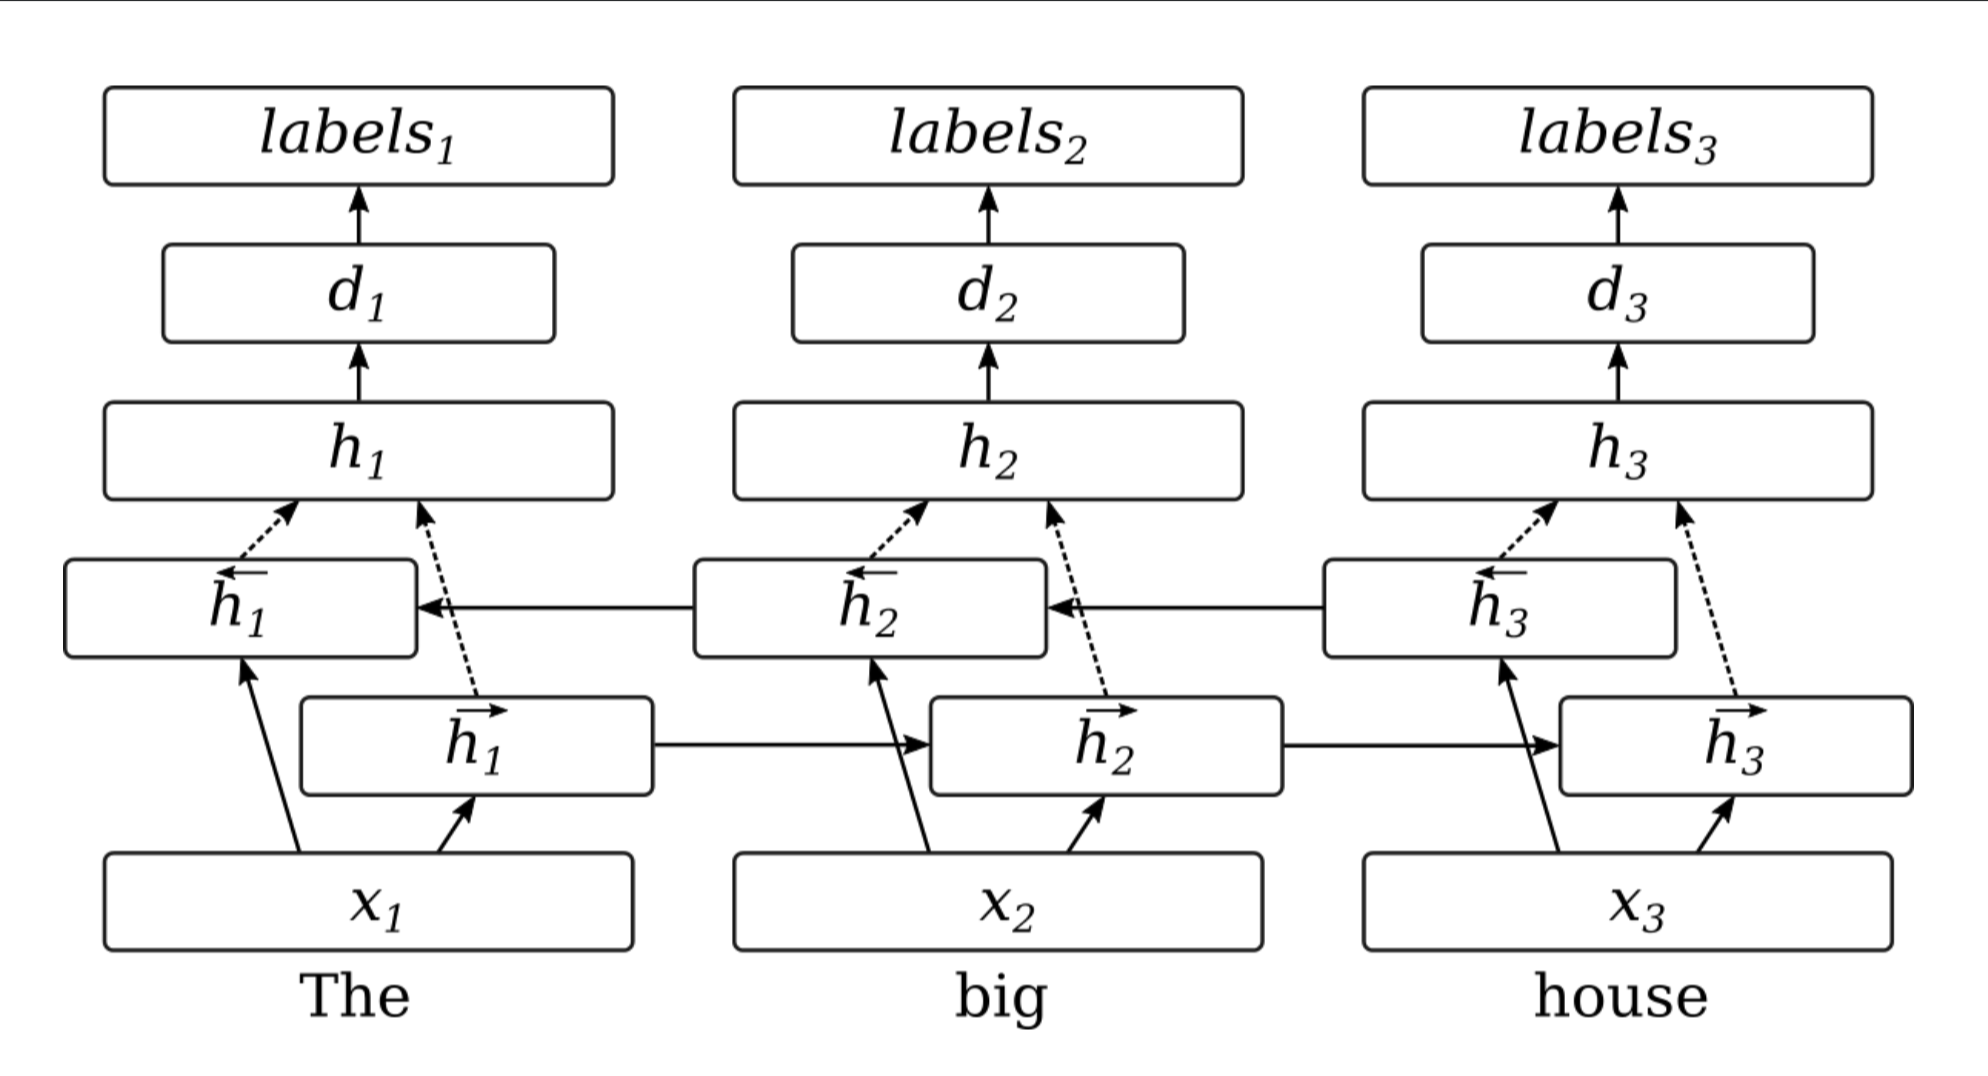
\includegraphics[width=0.7\textwidth]{./__pics/BiLSTM.eps}
	\caption{Схема базовой модели BiLSTM}
\end{figure}

Затем, добавляется скрытый слой нелинейности:
$$d_\text{t} = tanh(W_\text{d}h_\text{t}),$$
где $\textbf{W}_\text{d}$ -- весовая матрица между слоями.

В конце для создания самих меток используется либо softmax либо Conditional Random Fields (разновидность метода Марковских случайных полей) в зависимости от выбранной постановки задачи. Функция softmax рассчитывает нормированное распределение вероятностей по всем возможным меткам для каждого слова:

$$\mathbb{P}(y_t = k| d_t) = \cfrac{e^{W_kd_\text{t}}}{\sum_{\tilde{k}\in K}e^{W_\tilde{k}d_\text{t}}},$$
где $\mathbb{P}(y_t = k| d_t)$ -- вероятность того, что метка t-ого слова $y_t$ будет k ($K$ -- множество всевозможных меток), $\textbf{W}_k$ -- k-ая строка весовой матрицы $\textbf{W}$. 

Для оптимизации модели используется минимизация отрицательного логарифма вероятности верной метки: 
$$\mathcal{L} = -\sum_{t=1}^{T}\log(\mathbb{P}(y_t|d_t))$$


\paragraph{Усовершенствования базового алгоритма} 

\section{Результаты работы алгоритма}
Самый важный график



\section{Заключение}



\bibliographystyle{unsrt}
\bibliography{jmlda-bib}
\begin{thebibliography}{1}

\bibitem{author09anyscience}
    \BibAuthor{Marek Rei, Gamal K.O. Crichton,  Sampo Pyysalo \;N.}
    \BibTitle{Attending to Characters in Neural Sequence Labeling Models}~//
    \BibJournal{Proceedings of COLING 2016, the 26th International Conference on Computational Linguistics: Technical Papers }, 2016, C16-1030, Pp.\,309--318.

\bibitem{author09anyscience}
	\BibAuthor{Adnan Akhundov, Dietrich Trautmann, Georg Groh \;N.}
	\BibTitle{Sequence Labeling: A Practical Approach}~//
	\BibJournal{CoRR }, vol. abs/1808.03926, 2018.

\bibitem{author09anyscience}
	\BibAuthor{Zachary Chase Lipton, John Berkowitz \;N.}
	\BibTitle{A Critical Review of Recurrent Neural Networks for Sequence Learning }~//
	\BibJournal{CoRR }, vol. abs/1506.00019, 2015.

\bibitem{author09anyscience}
	\BibAuthor{Vaswani, Ashish and Shazeer, Noam and Parmar, Niki and Uszkoreit, Jakob and Jones, Llion and Gomez, Aidan N and Kaiser, \L ukasz and Polosukhin, Illia \;N.}
	\BibTitle{Attention is all you need }~//
	\BibJournal{Advances in Neural Information Processing Systems 30}, 2017, Pp.\,5998--6008.

\bibitem{author09anyscience}
	\BibAuthor{Adnan Akhundov, Dietrich Trautmann, Georg Groh \;N.}
	\BibTitle{LONG SHORT-TERM MEMORY}~//
	\BibJournal{Journal Neural Computation archive Volume 9 Issue 8 }, 1997, Pp.\,1735--1780 
%\bibitem{myHandbook}
%    \BibAuthor{Автор\;И.\,О.}
%    Название книги.
%    Город: Издательство, 2009. 314~с.
%\bibitem{author09first-word-of-the-title}
%    \BibAuthor{Автор\;И.\,О.}
%    \BibTitle{Название статьи}~//
%    \BibJournal{Название конференции или сборника},
%    Город:~Изд-во, 2009.  С.\,5--6.
%\bibitem{author-and-co2007}
%    \BibAuthor{Автор\;И.\,О., Соавтор\;И.\,О.}
%    \BibTitle{Название статьи}~//
%    \BibJournal{Название журнала}. 2007. Т.\,38, \No\,5. С.\,54--62.
%\bibitem{bibUsefulUrl}
%    \BibUrl{www.site.ru}~---
%    Название сайта.  2007.
%\bibitem{voron06latex}
%    \BibAuthor{Воронцов~К.\,В.}
%    \LaTeXe\ в~примерах.
%    2006.
%    \BibUrl{http://www.ccas.ru/voron/latex.html}.
%\bibitem{Lvovsky03}
%    \BibAuthor{Львовский~С.\,М.} Набор и вёрстка в пакете~\LaTeX.
%    3-е издание.
%    Москва:~МЦHМО, 2003.  448~с.
\end{thebibliography}

% Решение Программного Комитета:
%\ACCEPTNOTE
%\AMENDNOTE
%\REJECTNOTE
\end{document}
